\begin{frame}\frametitle{ \vspace*{0.5cm} Results: Dependence on the length of the wave}
  \begin{figure}
    \centering
    \hfill%
    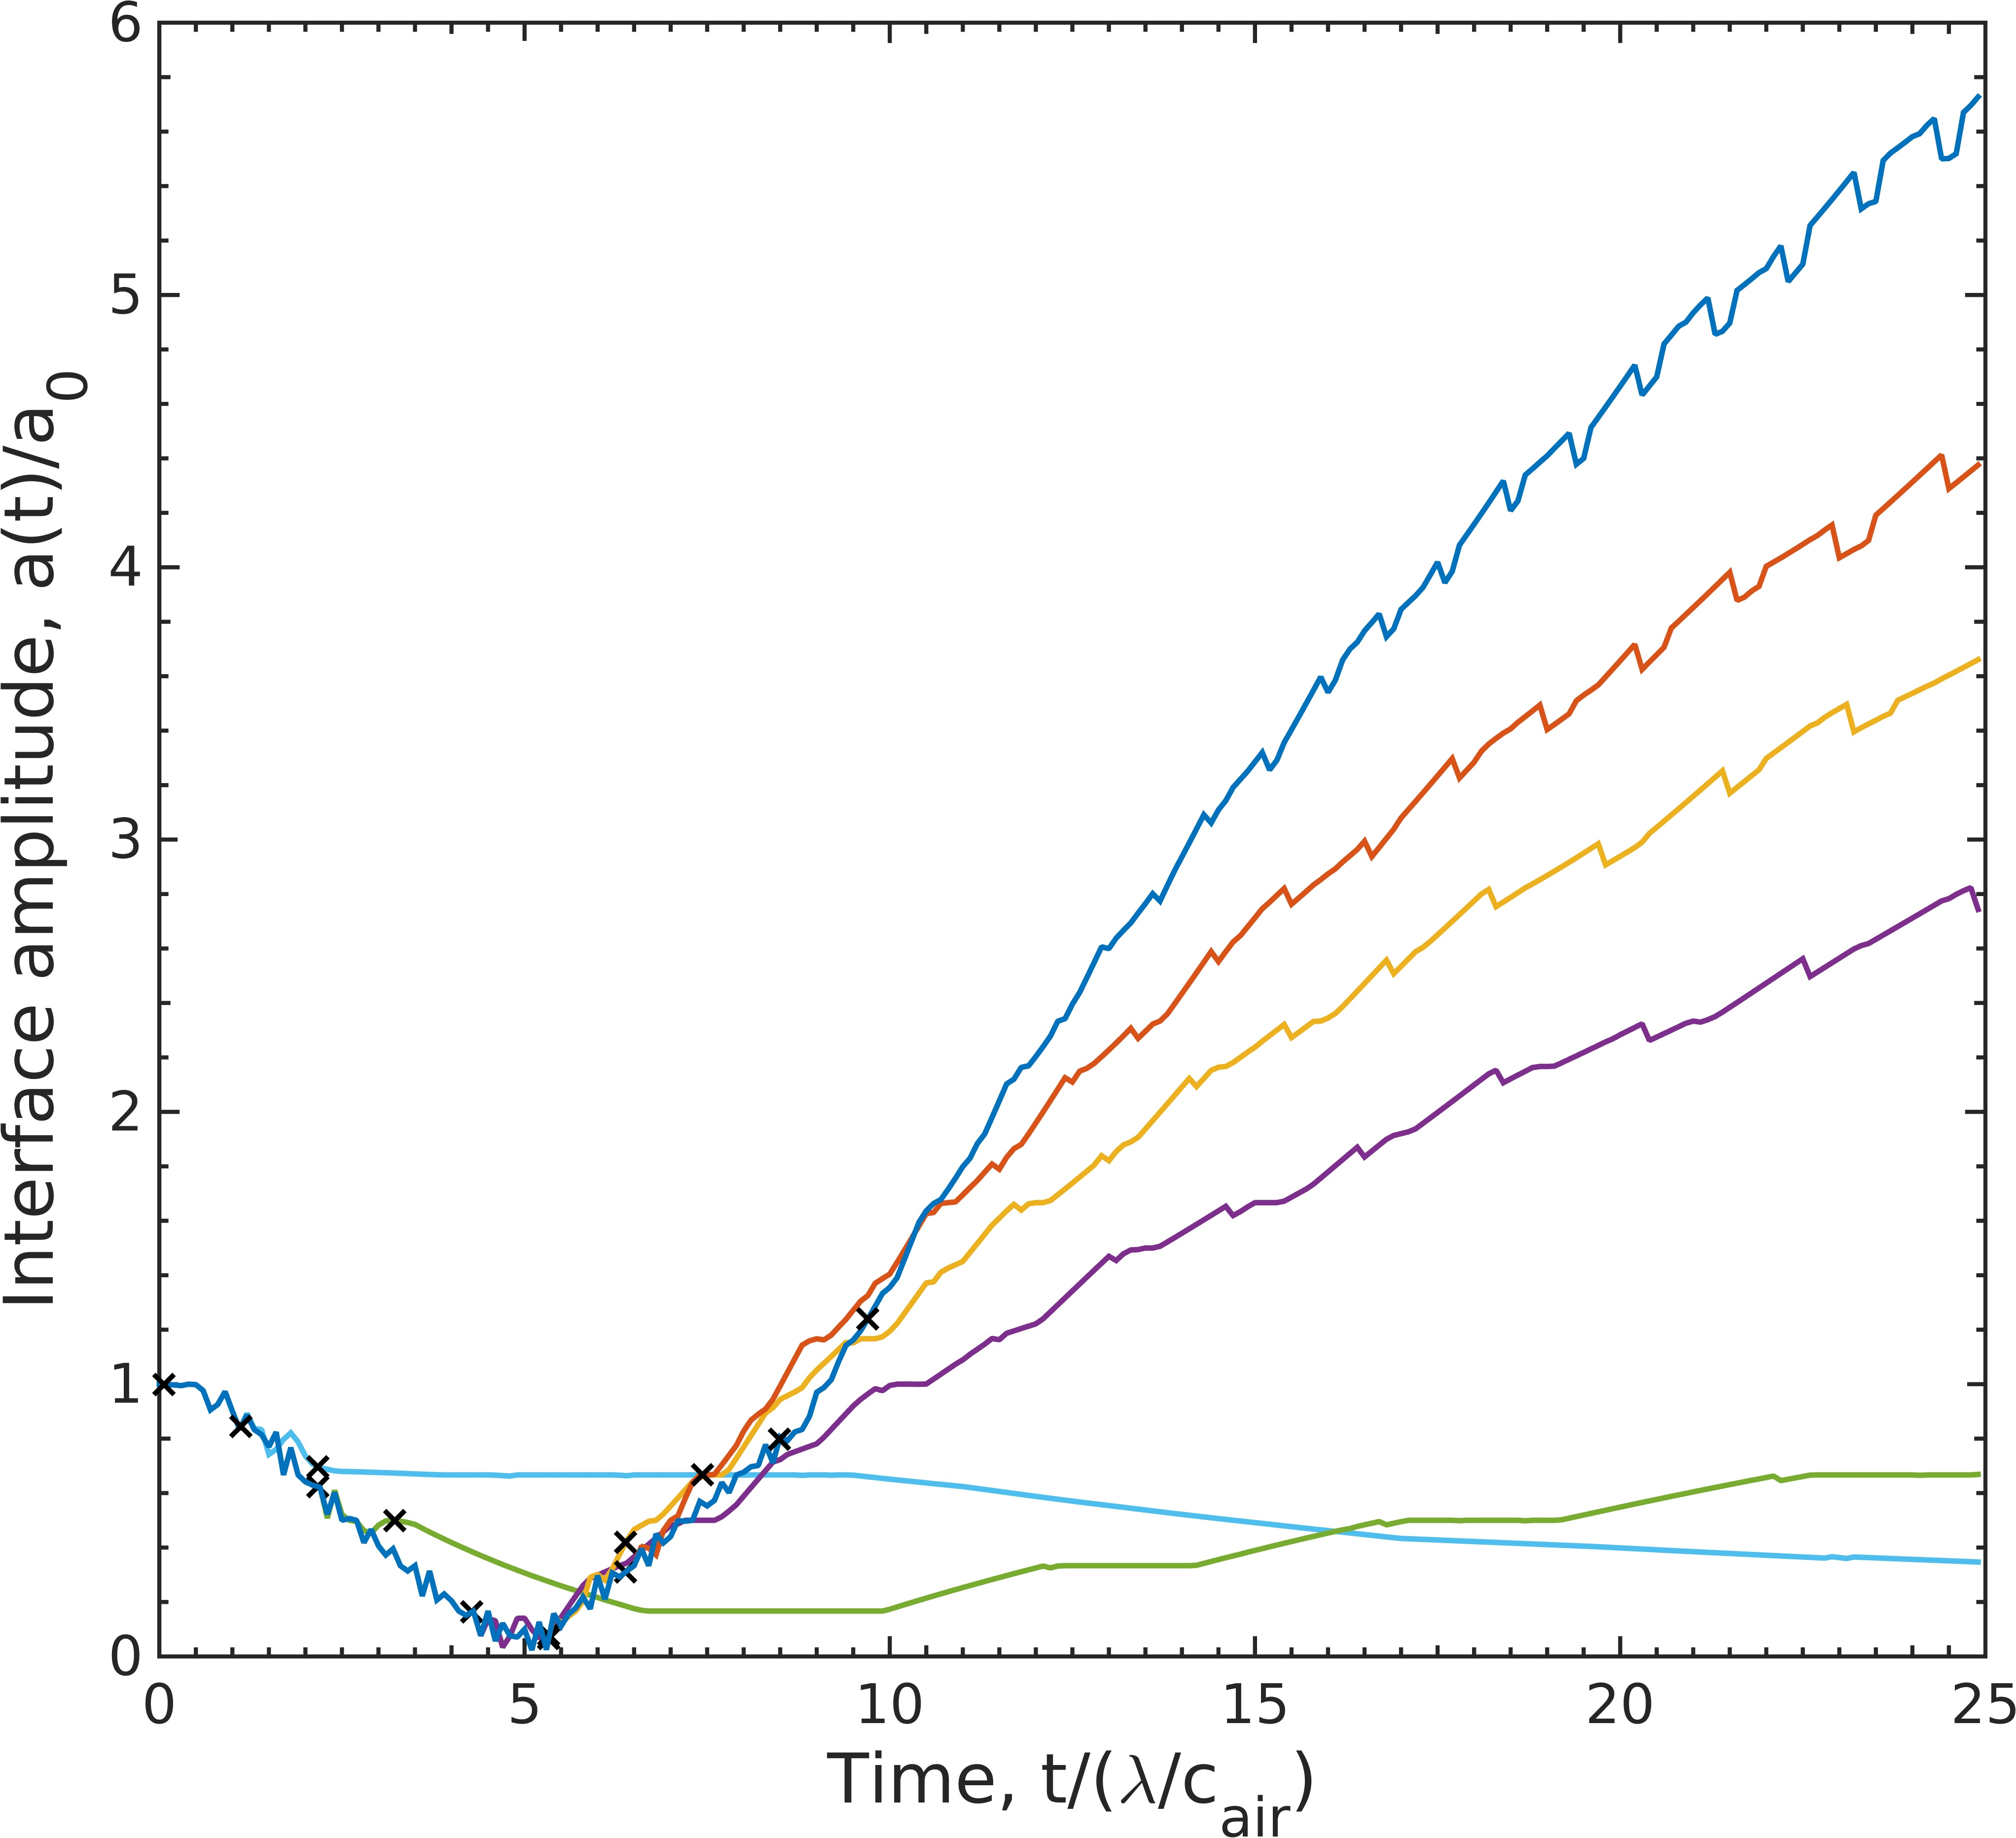
\includegraphics[height=0.52\textheight]{../figs/lung_figs/interface_multi-lag}\hfill%
    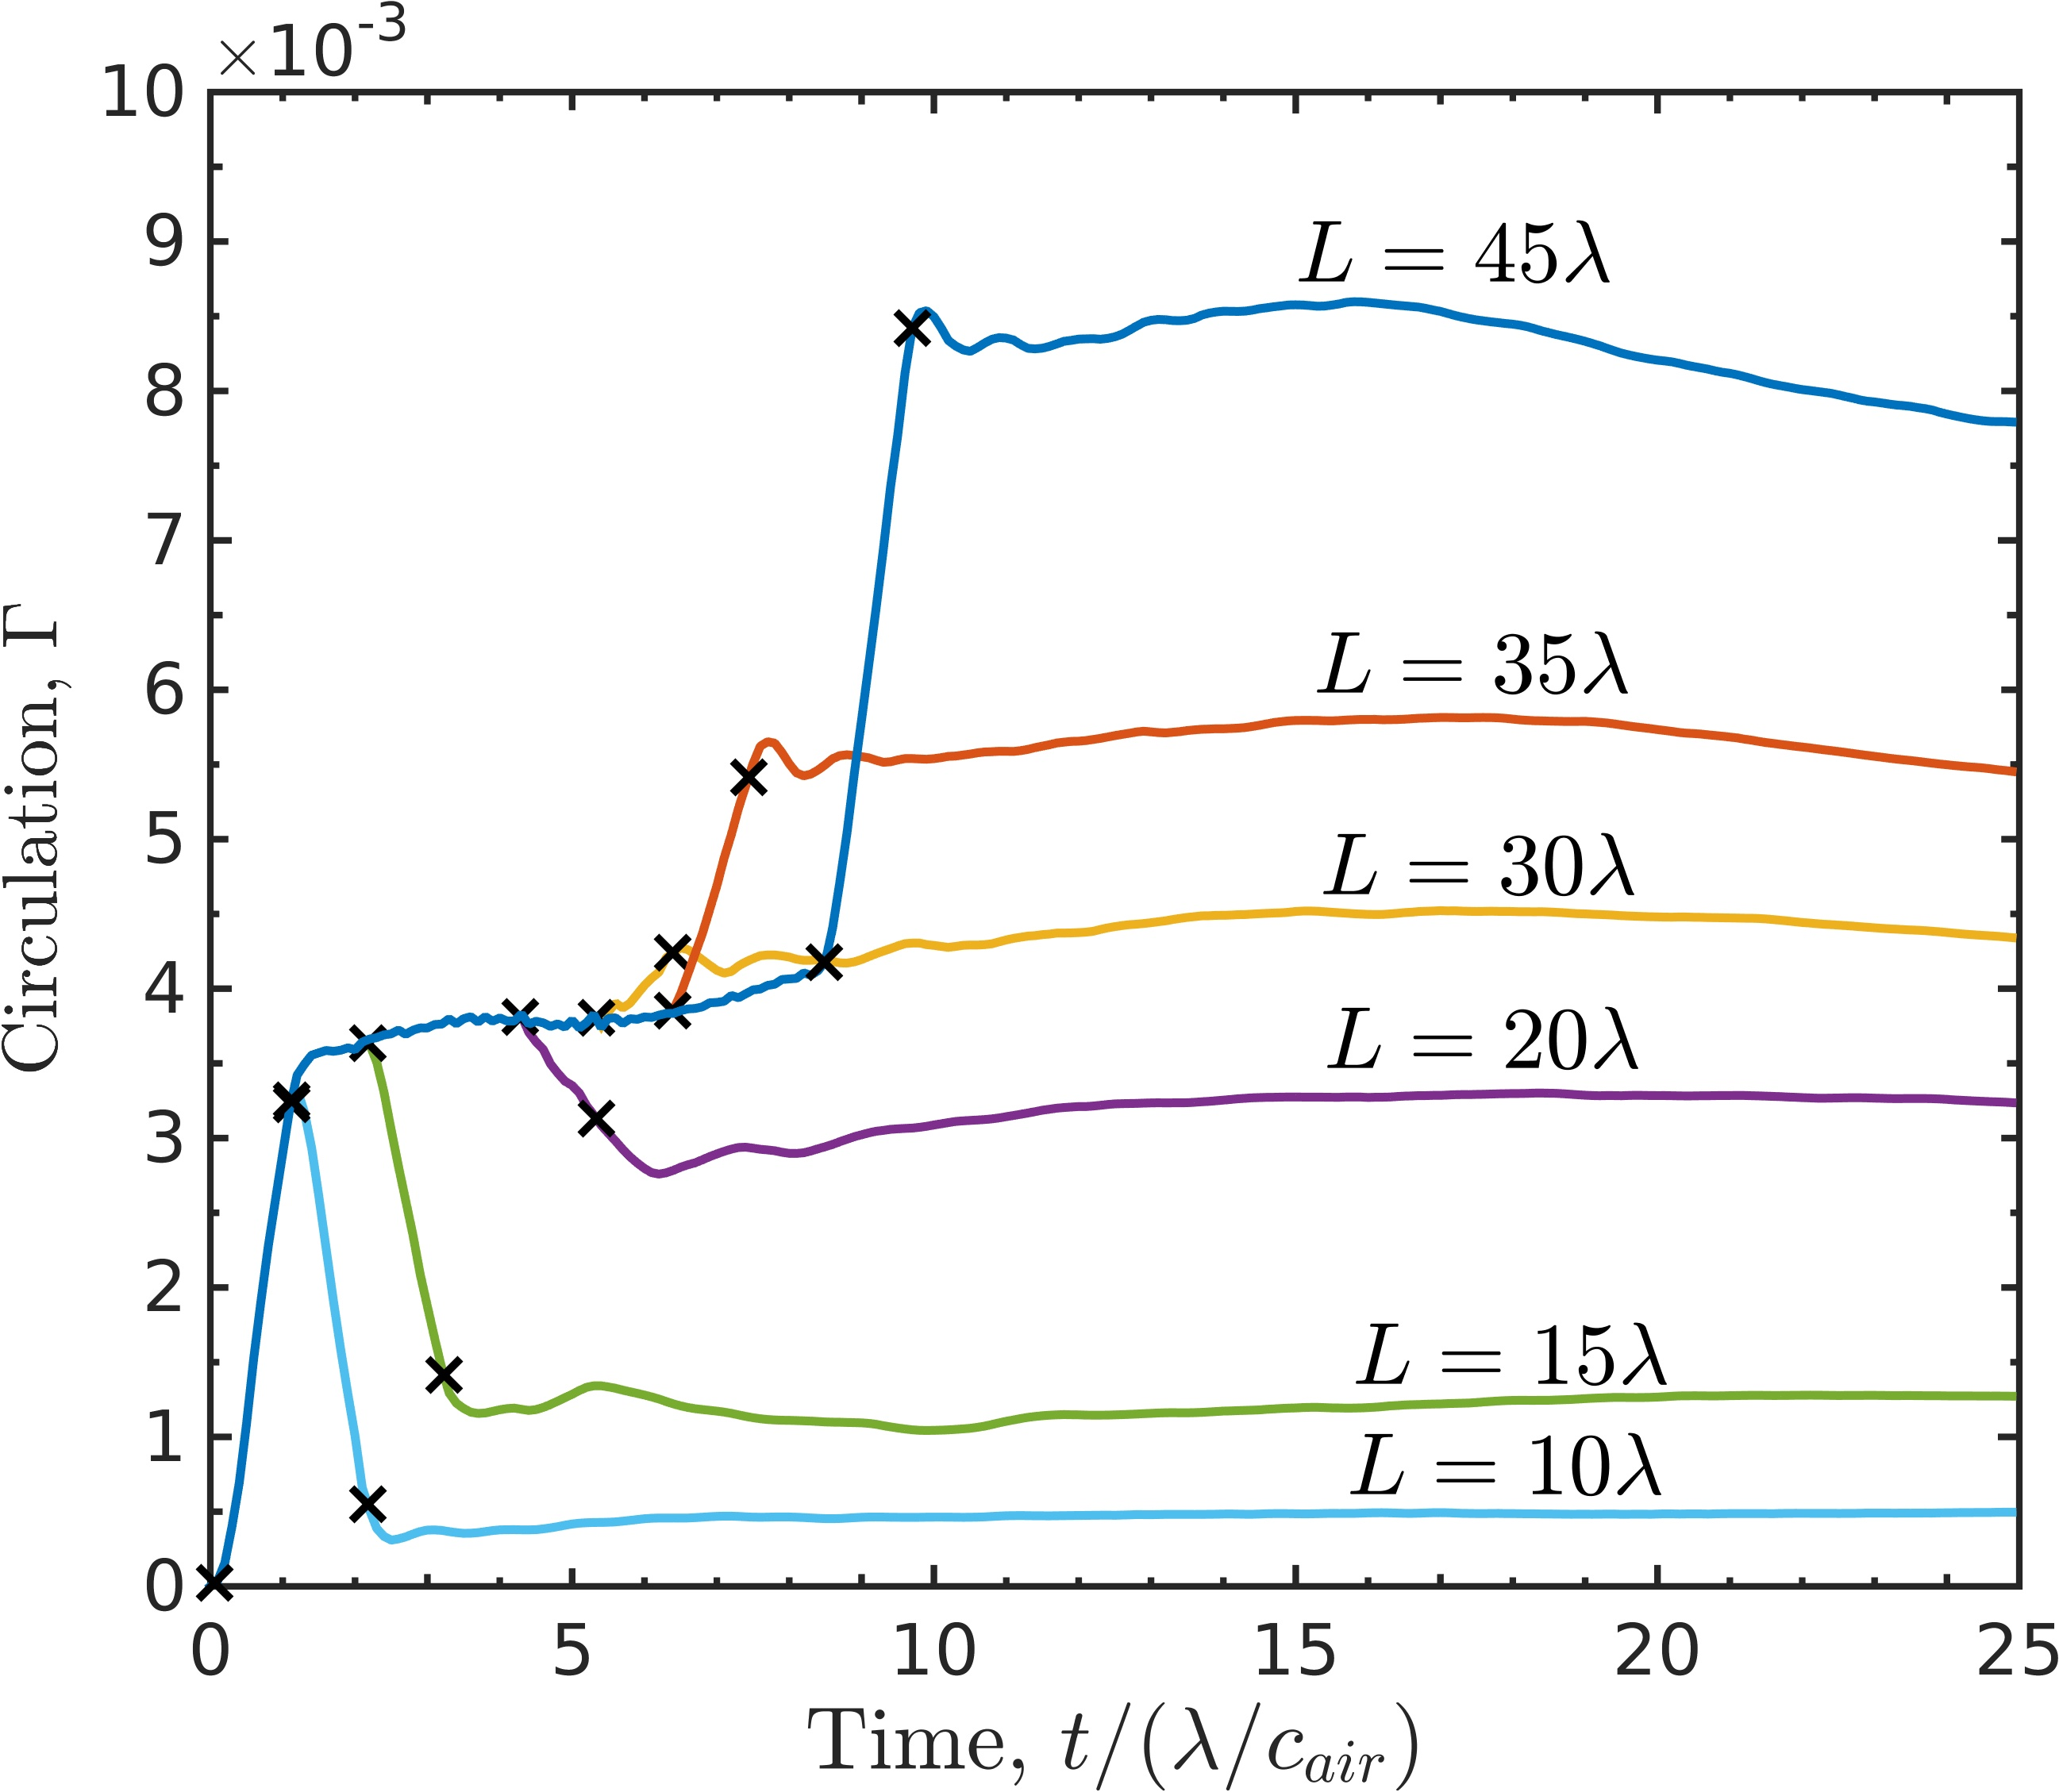
\includegraphics[height=0.53\textheight]{../figs/lung_figs/circulation_multi-lag_fixed}%
    \hfill%
  \end{figure}
  \begin{itemize}
  \item Changing wave width changes time when expansion hits interface.
  \item Time-dependent interface deformation causes time-dependent vorticity deposition.
  \item The long-term interface dynamics can change appreciably.
  \end{itemize}

  %
  \note{
    To Do: Remove
    un-neccessary lines, $15\lambda$,
    Mauro's Questions:\\
    \begin{itemize}
    \item Is there a way to non-dimensionalize this show that the
      transition of the physics occurs between $L = 20 - 30 \lambda$.\\
      This essentially boils down to figuring out the speed of
      the interface evolution and modeling the time at which the
      phase-inversion will occur.\\Maybe I should subtract
      $\Delta L_{lag}$ to see this better, or divide $\gamma$ by
      $a(t=t_{phase-reversal})^n$ or $\Delta L_{Lag}^n$.\\
    \item What is the Reynolds number?
    \end{itemize}

  }
\end{frame}
%%% Local Variables:
%%% mode: latex
%%% TeX-master: "../main"
%%% End:
